\documentclass[11pt,letterpaper]{article}

\newenvironment{proof}{\noindent{\bf Proof:}}{\qed\bigskip}

\newtheorem{theorem}{Theorem}
\newtheorem{corollary}{Corollary}
\newtheorem{lemma}{Lemma} 
\newtheorem{claim}{Claim}
\newtheorem{fact}{Fact}
\newtheorem{definition}{Definition}
\newtheorem{assumption}{Assumption}
\newtheorem{observation}{Observation}
\newtheorem{example}{Example}
\newcommand{\qed}{\rule{7pt}{7pt}}

\newcommand{\solution}[4]{
\thispagestyle{plain} 
\newpage
\setcounter{page}{1}
\noindent
\begin{center}
\framebox{ \vbox{
\vspace{4mm}
\vspace{0.2in} 
{\centering \large\mbox{#3}}\\
\vspace{0.1in}
{#1 \hfill {Date: #2}}
}}
\end{center}
\markright{#1}
}

\newenvironment{algorithm}
{\begin{center}
\begin{tabular}{|l|}
\hline
\begin{minipage}{1in}
\begin{tabbing}
\quad\=\qquad\=\qquad\=\qquad\=\qquad\=\qquad\=\qquad\=\kill}
{\end{tabbing}
\end{minipage} \\
\hline
\end{tabular}
\end{center}}

\def\Comment#1{\textsf{\textsl{$\langle\!\langle$#1\/$\rangle\!\rangle$}}}


\usepackage{graphicx}
\usepackage{float}
\usepackage{multicol}
\usepackage{balance}
\usepackage{multicol}
\usepackage{multirow}
\usepackage{epstopdf}
\usepackage{epsfig}
\usepackage{makeidx}
\usepackage{bm}
\usepackage{pbox}
\usepackage{pdflscape}
\usepackage{url}
\usepackage{framed}
\usepackage{mathtools}
\usepackage{adjustbox}
\usepackage{amsmath}
\usepackage{hyperref}
\usepackage{subcaption}
\usepackage{cite}
\usepackage{amsfonts}

\usepackage{graphicx, amssymb, amsmath, listings, float, mathtools}
\usepackage{color, url}
\lstset{language = Python}
\lstset{breaklines}
\lstset{extendedchars=false}

\oddsidemargin 0in
\evensidemargin 0in
\textwidth 6.5in
\topmargin -0.6in
\textheight 9.0in

\begin{document}

\solution{\large Jifu Zhao}{\large 02/18/2018}{\bf \Large STAT 578  \hspace{0.5cm} 
		Spring 2018 \hspace{0.5cm} Homework 1}


\section*{(a)}

The given dataset is Movielens 100K, which contains 943 users and 1682 movies in total. The given dataset has been splitted into 5 folders, and forms 5 different training and test set, named (u1\_base, u1\_test), (u2\_base, u2\_test), (u3\_base, u3\_test), (u4\_base, u4\_test), (u5\_base, u5\_test). In addition to the userID, itemID, rating information, we also have the information about each user as well as each item. 

For the first question, I explored two models. The first model is simply linear regression. In this model, we treat each user and each item's information as the predictor, including age, gender, item category and so on, train the model using the training set, and make predictions on the test set. 

In addition to the linear regression model, we also implement KNN model using the Surprise package, which is a Python package for building and analyzing recommender systems. We choose the item-based KNN algorithm. 

The performance of two algorithms is shown in Table~\ref{result}

\begin{table}[htbp]
 \caption{Summary of Cross Validation} \label{result}
 \vspace{0.1in}
\begin{center}
  \begin{tabular}{  c  c  c}
    \hline
    RMSE/Model        & Linear Regression        & KNN      \\ \hline
    CV 1                     & 1.13332                           & 1.15368 \\ \hline
    CV 2                    & 1.11352                            & 1.13066 \\ \hline
    CV 3                    & 1.09645                           & 1.11158 \\ \hline
    CV 4                    & 1.09598                           & 1.11329 \\ \hline
    CV 5                    & 1.09997                           & 1.11868  \\ \hline
    Mean                   & 1.10785                           &  1.12558 \\ \hline 
    Std                      & 0.01424                           &  0.01556 \\ \hline 
  \end{tabular}
\end{center}
\end{table}

\section*{(b)}

In this part, we implement a series of visualization tools to infer the behaviour of the missing ratings.

Based on the user, item, and rating information, we can construct the utility matrix, where rows correspond to users, columns correspond to items, and the colors correspond to user's rating on specific item. For the missing ratings, we fill it with 0. The utility matrix is shown in Figure~\ref{fig:utility}.

\begin{figure}[htbp]
\centering
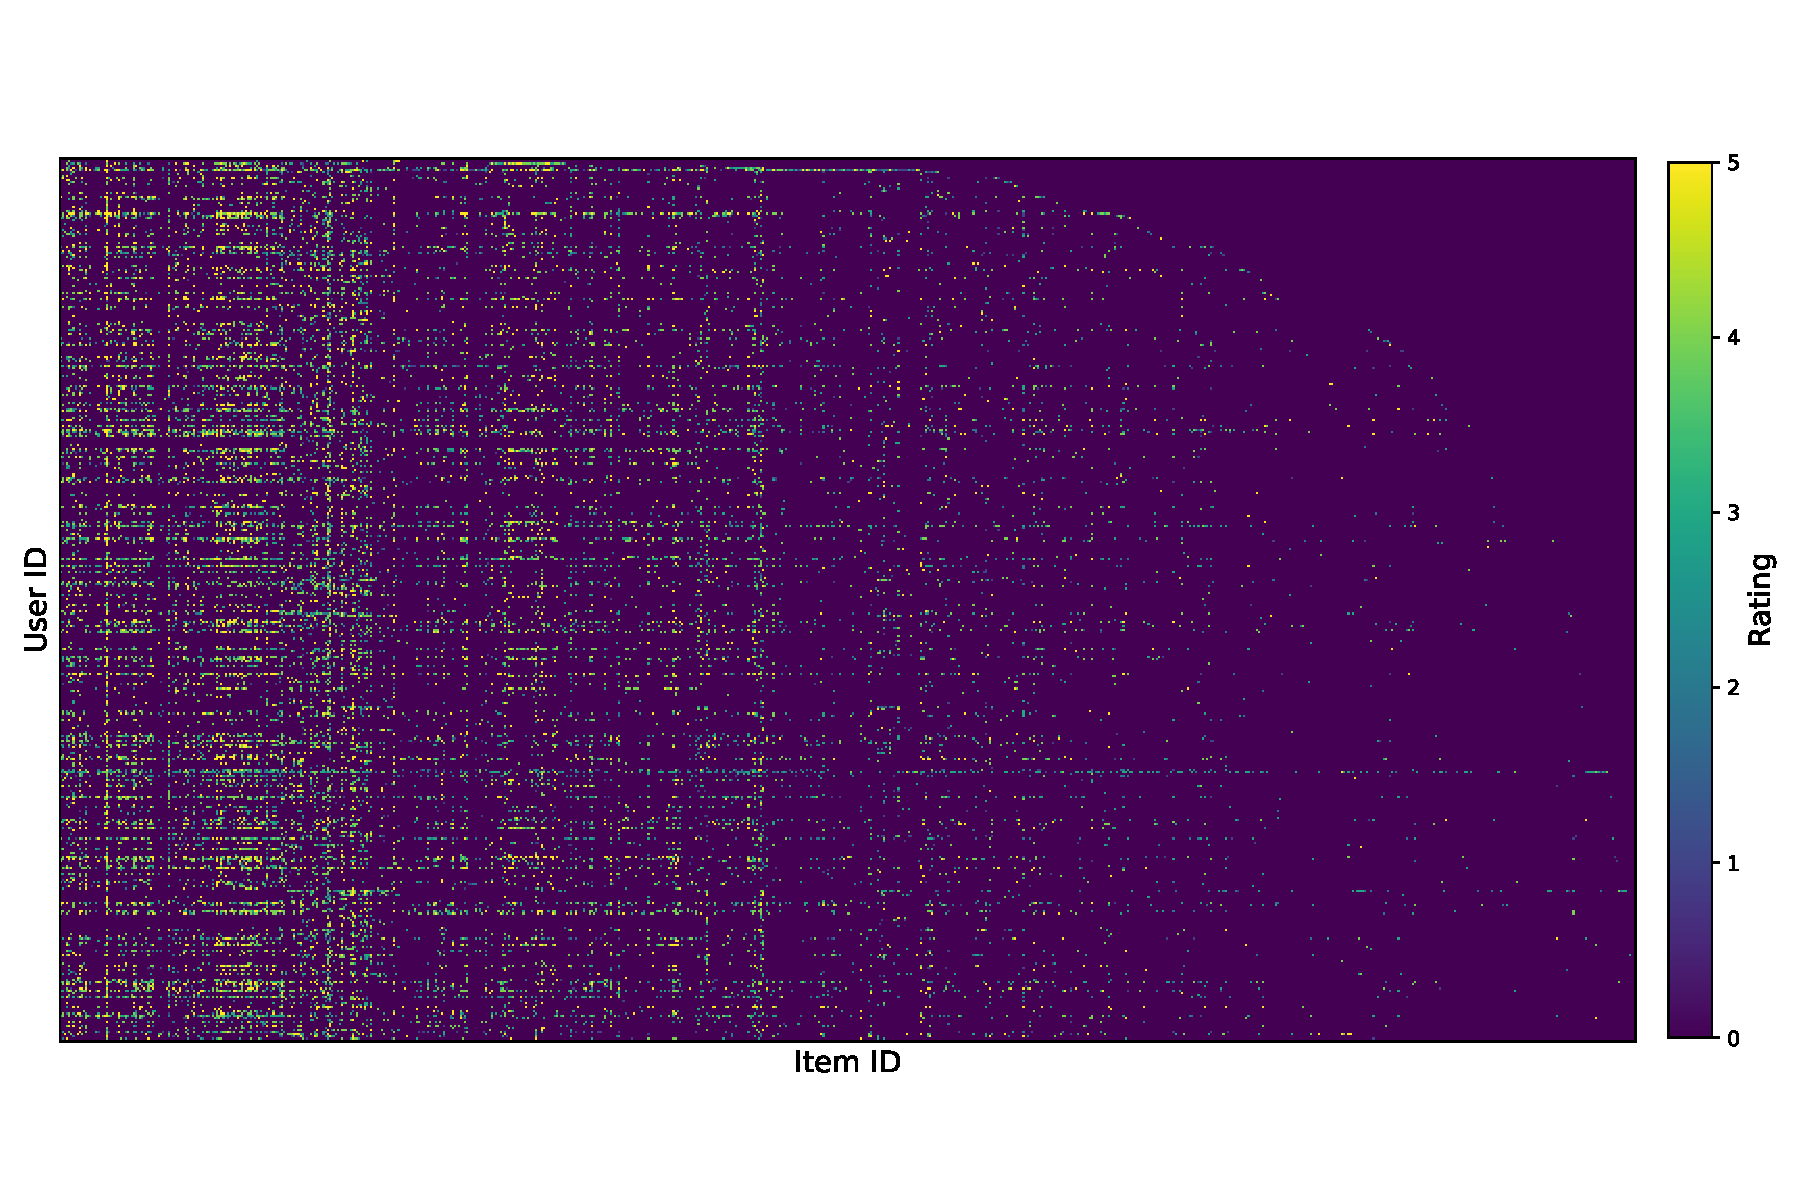
\includegraphics[width=1.0\textwidth]{./figures/utility.pdf}
\caption{User-item utility matrix}
\label{fig:utility} 
\end{figure}

From Figure~\ref{fig:utility}, we can see that, the missing ratings are not occur at random. For movies that have high ratings, there are less missing values. On the other hand, for movies that have relative low ratings, there are more missing values. 

\begin{figure}[htbp]
\centering
\begin{subfigure}[b]{0.5\linewidth}
  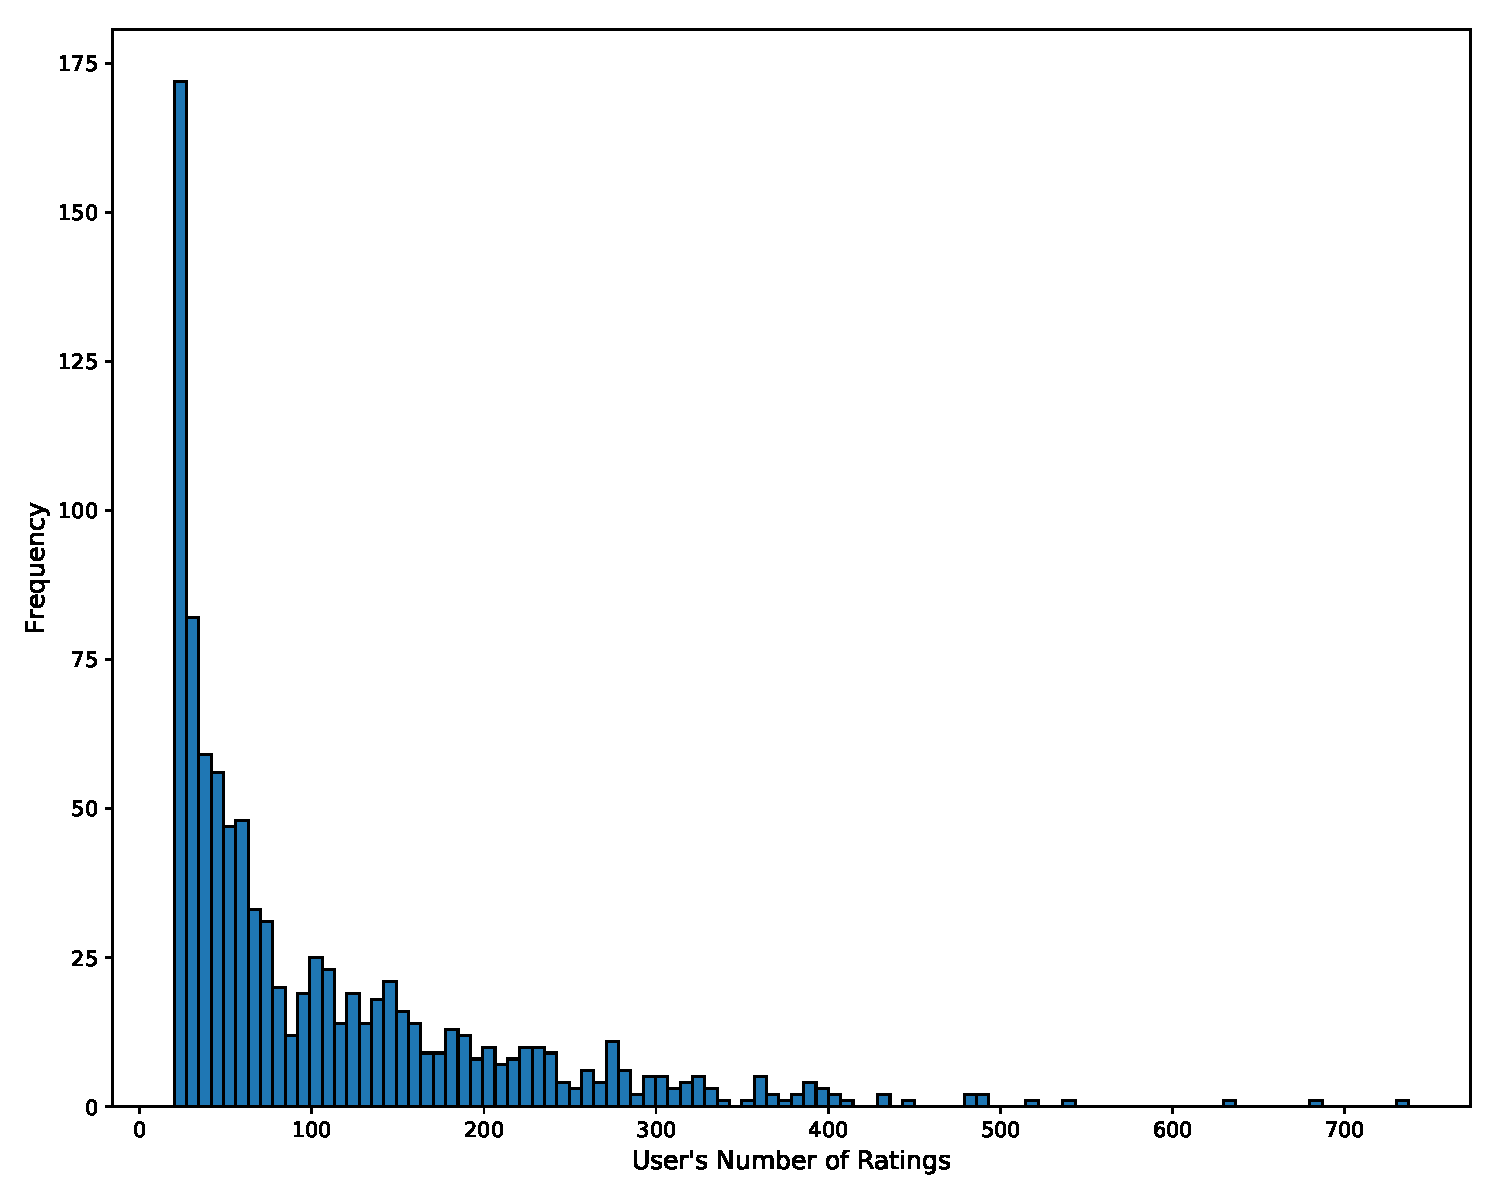
\includegraphics[width=1.00\textwidth]{./figures/user_frequency.pdf}
  \caption{Distribution of user's number of ratings}
   \label{ex_without_source}
\end{subfigure}%
\begin{subfigure}[b]{0.5\linewidth}
  \centering
  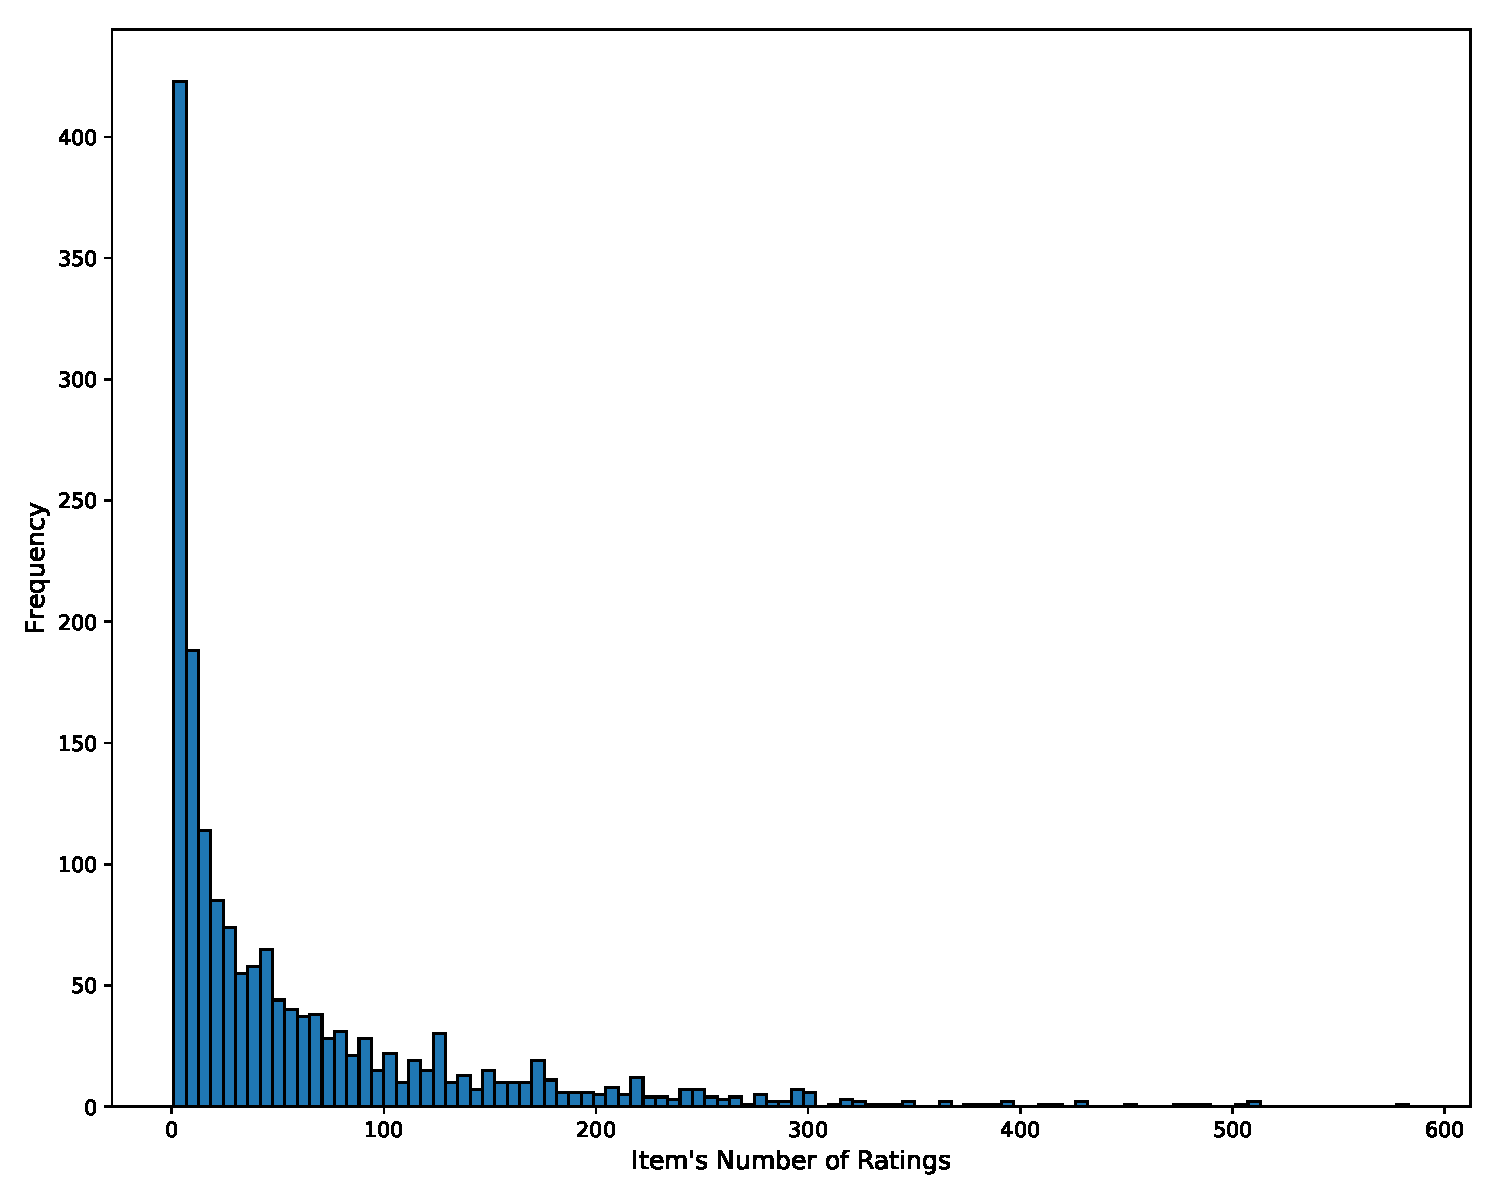
\includegraphics[width=1.00\textwidth]{./figures/item_frequency.pdf}
  \caption{Distribution of item's number of ratings}
  \label{ex_with_source}
\end{subfigure}%
\raggedright
\caption{Distribution of User's / Item's number of ratings}
\label{fig:source_injection1}
\end{figure}

\newpage
To see more details, we plot the distribution of user's and item's number of ratings in Figure~\ref{fig:source_injection1}. As shown clearly, most users and most movies have low number of ratings. The distributions show long tails for high number of ratings.

In addition to the distribution of number of ratings, we also plot the relation of user's or item's mean rating versus the number of ratings. As shown in Figure~\ref{fig:source_injection2}, for users, their mean rating are mainly normally distributed. On the other hand, for movies, the movies who have relatively higher number of ratings, tend to have relative higher mean rating.

\begin{figure}[!h]
\centering
\begin{subfigure}[b]{0.5\linewidth}
  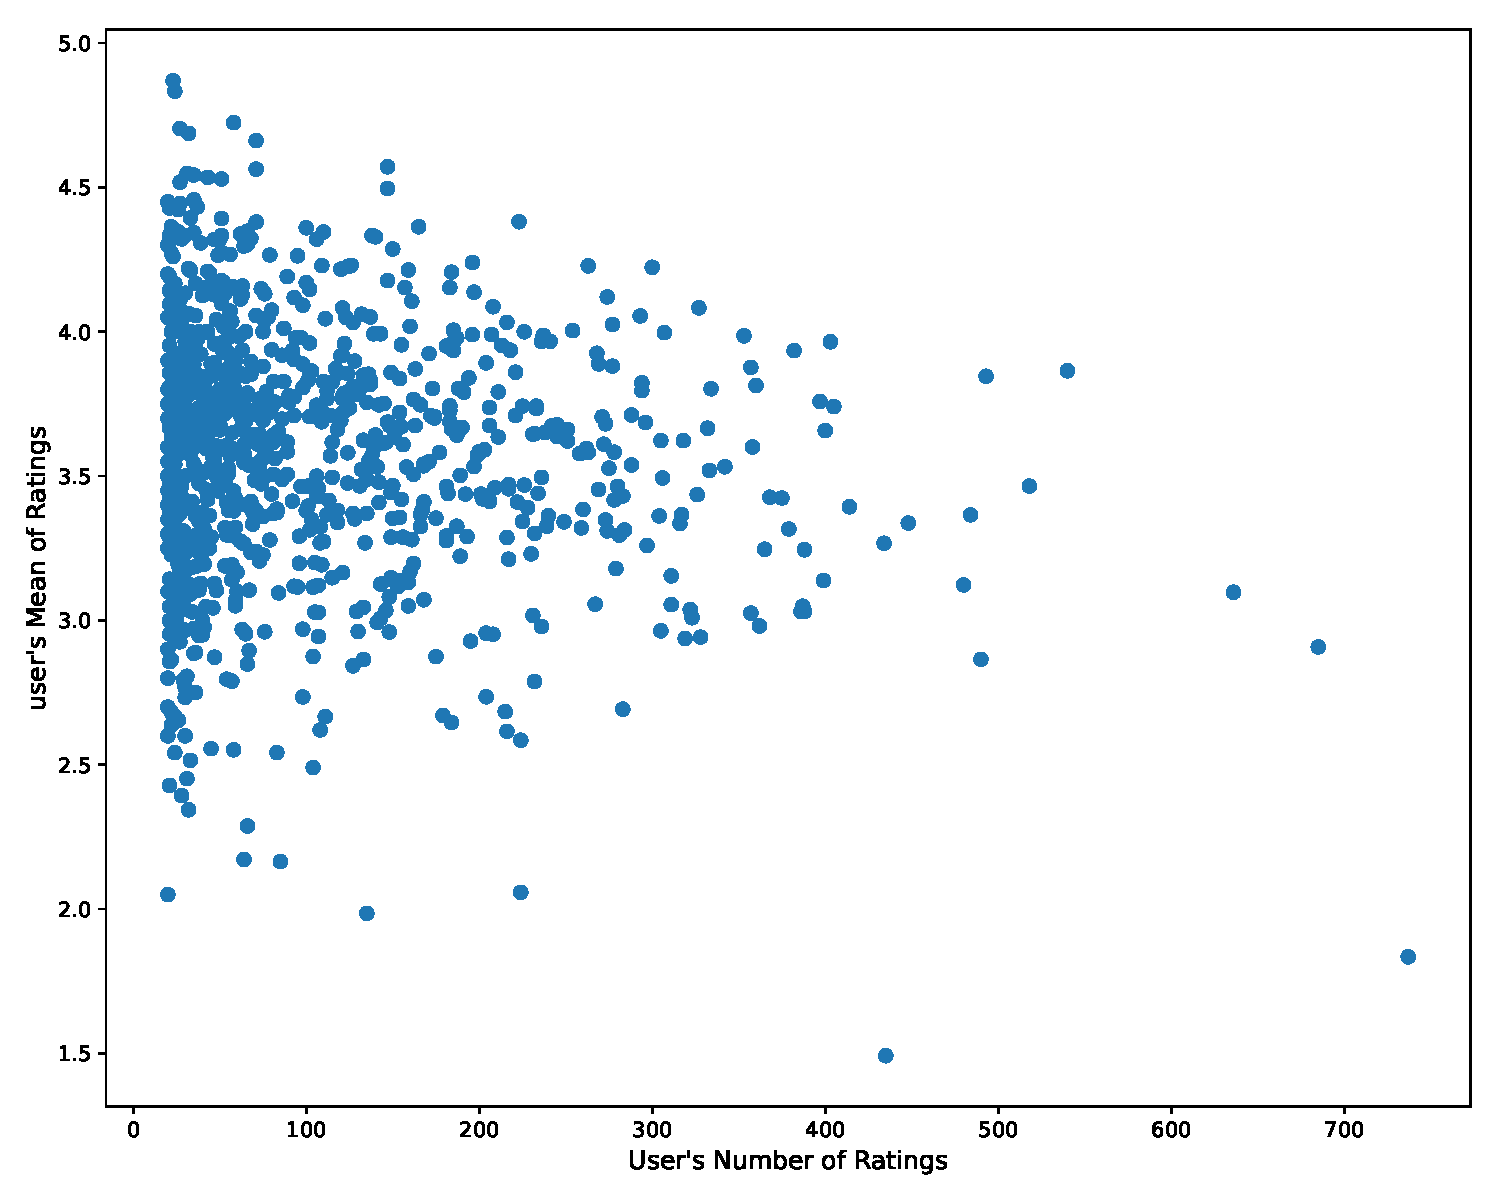
\includegraphics[width=1.00\textwidth]{./figures/user_mean_rating.pdf}
  \caption{User's mean rating vs. number of ratings}
   \label{ex_without_source}
\end{subfigure}%
\begin{subfigure}[b]{0.5\linewidth}
  \centering
  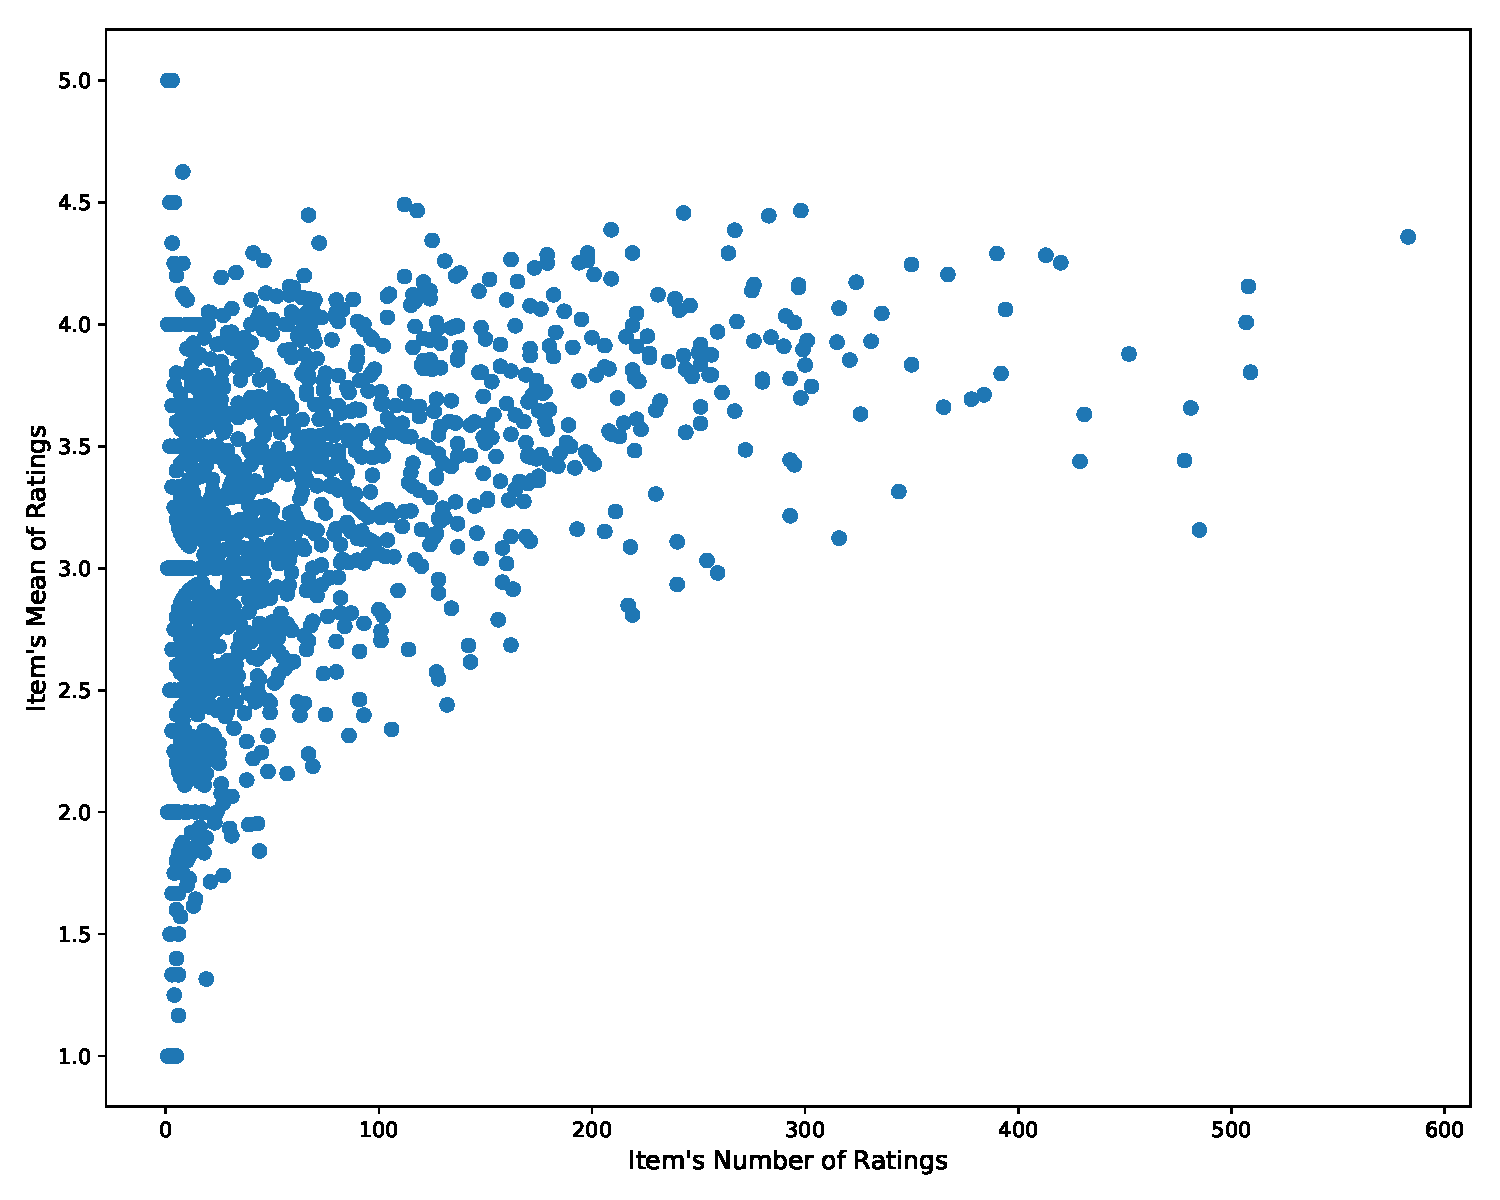
\includegraphics[width=1.00\textwidth]{./figures/item_mean_rating.pdf}
  \caption{Item's mean rating vs. number of ratings}
  \label{ex_with_source}
\end{subfigure}%
\raggedright
\caption{Mean ratings vs. number of ratings}
\label{fig:source_injection2}
\end{figure}

\section*{(c)}
Based on our analysis in Part (c), we can notice one clear phenomenon, for movies with relatively larger number of ratings, there tend to have relatively higher mean ratings. Based on this, we can use the number of ratings for each movie to indicate its popularity. In Figure~\ref{fig:fitted}, we fit a linear curve for mean rating and number of ratings.

\begin{figure}[htbp]
\centering
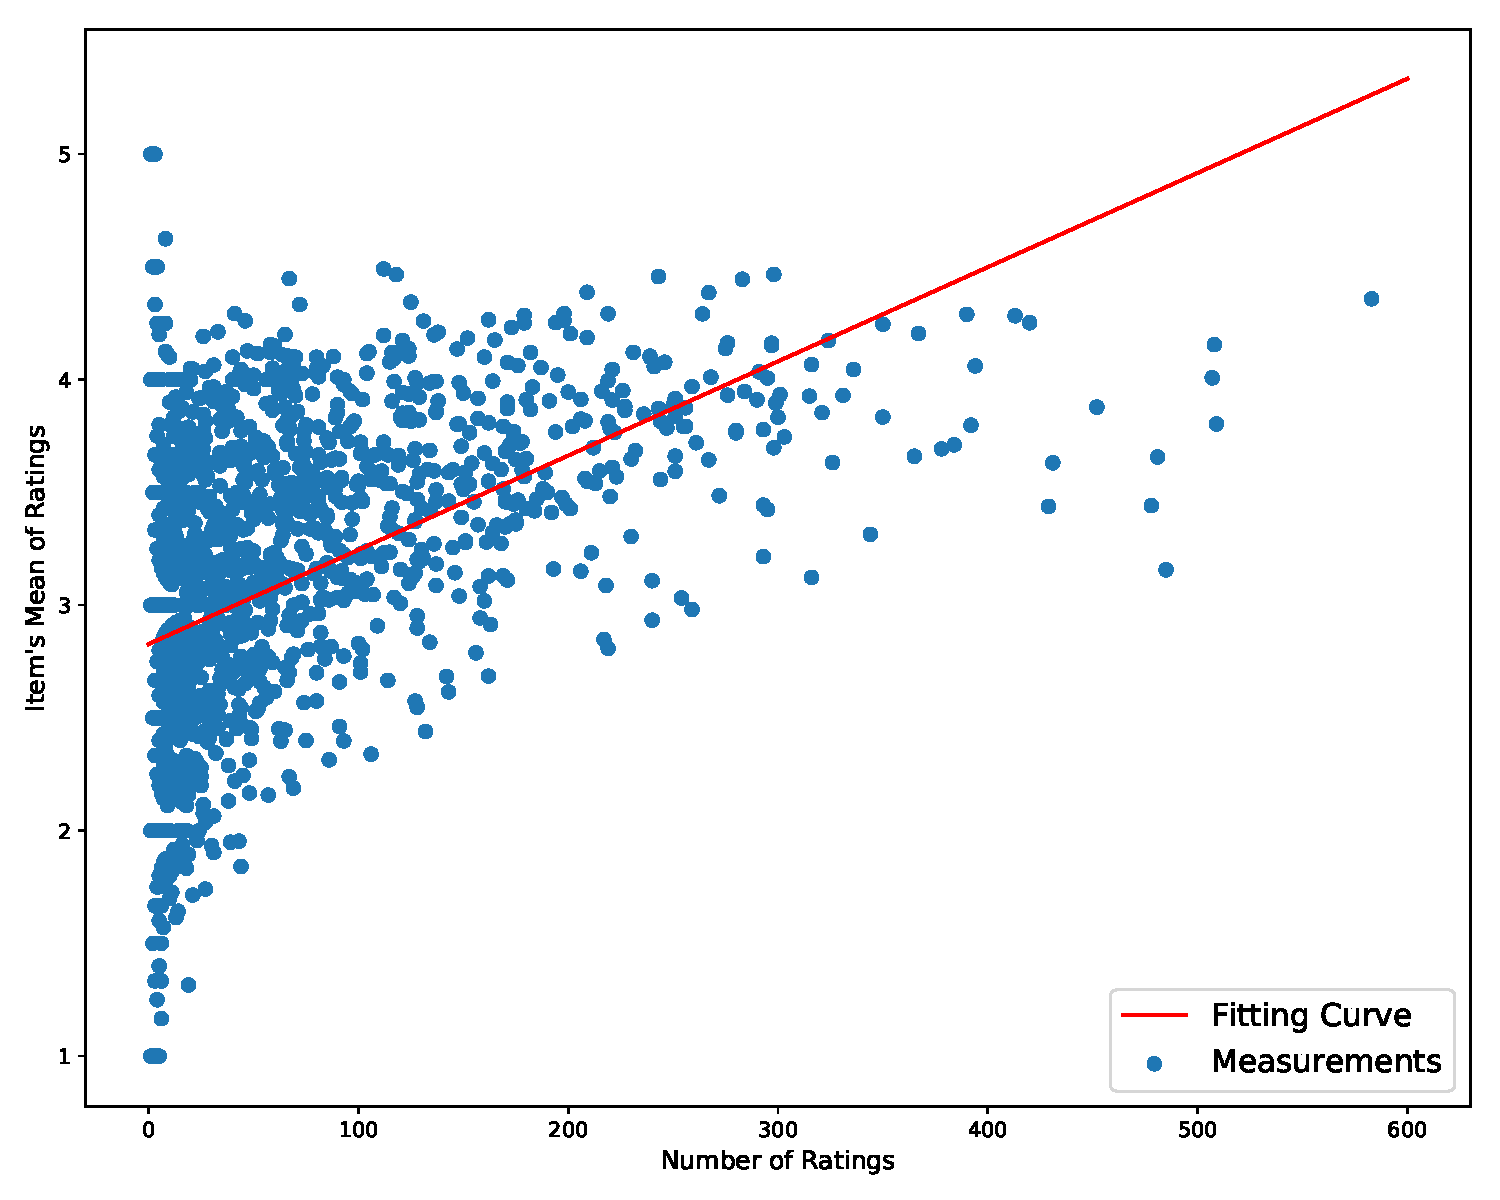
\includegraphics[width=0.8\textwidth]{./figures/fitting_curve.pdf}
\caption{Item's mean of ratings vs. number of ratings}
\label{fig:fitted} 
\end{figure}

To improve the performance of the prediction, we re-build the linear regression model and the item-based KNN model. This time, for linear regression model, we add another feature corresponding to popularity (in actual code, we use the fitted mean rating to represent the popularity, instead of using the raw number of ratings). For KNN model, in addition to the prediction from KNN model, we choose the average value of KNN's prediction and the mean value from fitted curve in Figure~\ref{fig:fitted} as the final prediction. All the results are shown in Table~\ref{result2}.


\begin{table}[htbp]
 \caption{Summary of Cross Validation} \label{result2}
 \vspace{0.1in}
\begin{center}
  \begin{tabular}{  c  c  c}
    \hline
    RMSE/Model        & Linear Regression        & KNN     \\ \hline
    CV 1                     & 1.10348                           & 1.12234 \\ \hline
    CV 2                    & 1.08674                           & 1.10264 \\ \hline
    CV 3                    & 1.07505                           & 1.08820 \\ \hline
    CV 4                    & 1.07059                           & 1.08572 \\ \hline
    CV 5                    & 1.07674                           & 1.09375 \\ \hline
    Mean                   & 1.08252                           &  1.09853 \\ \hline 
    Std                      &  0.01173                           &  0.01325 \\ \hline 
  \end{tabular}
\end{center}
\end{table}

As shown clearly in Table~\ref{result2}, compared with Table~\ref{result}, both linear regression model and the KNN model give better results. More specifically, for linear regression model, the mean RMSE gets improved from 1.10785 to 1.08252, and for KNN model, the RMSE gets improved from 1.12558 to 1.09853.


\clearpage

%\bibliographystyle{plain}
%\bibliographystyle{unsrt}
%\bibliography{reference.bib}

\end{document}

